\documentclass[conference]{IEEEtran}
\IEEEoverridecommandlockouts
% The preceding line is only needed to identify funding in the first footnote. If that is unneeded, please comment it out.
\usepackage{cite}
\usepackage{amsmath,amssymb,amsfonts}
\usepackage{graphicx}
\usepackage{textcomp}
\usepackage{xcolor}
\def\BibTeX{{\rm B\kern-.05em{\sc i\kern-.025em b}\kern-.08em
T\kern-.1667em\lower.7ex\hbox{E}\kern-.125emX}}
\title{
\vspace{1cm}
{
\includegraphics[width=0.15\textwidth]{1.jpg} \\ Assembly Assignment}}
\author{AKHILA THALLA \\ Roll No: FWC22312 \\ akhilathalla0104@gmail.com}
\begin{document}
\maketitle
\section{ABSTRACT}
The Karnaugh map represents a logic function f. The minimal sum-of-products expression for f is derived by identifying the prime implicants and essential prime implicants in the Karnaugh map. The resulting expression is a simplified representation of the logic function, minimizing the number of literals and logic gates required for implementation.
\begin{figure}[h]
\centering
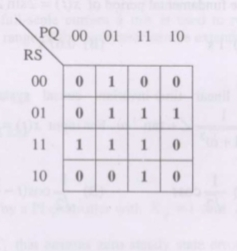
\includegraphics[width=0.5\textwidth]{2.jpg  }
\caption{\label{fig-1:Gates}}
\end{figure}
\section{COMPONENTS}
 The required components list is given in Table:I.,
 \vspace{0.3cm}
 \begin{table} [htbp]
 \centering
 \begin{tabular}{| c | c | c |} \hline
 components & value & quality \\ \hline
 Led's & & 4 \\ \hline
 Arduino & UNO & 1 \\ \hline
 jumperwires & & 50 \\ \hline
 Breadboard & & 1 \\
 \hline
 \end{tabular}
 \vspace{0.3cm}
 \caption{\label{tab:widgets}}
 \end{table}
 \section{PROCEDURE}
 \begin{enumerate}
 \item Connect the Led's to the Arduino uno.
 \item Give the inputs manually using jumper wires.
 \item connect the Arduino using USB device.
 \item Execute the arduino code in nvim editor using avra filename.tex command.
 \item After upload the code into hardware setup using arduino IDE platform.
 \end{enumerate}
 \section{RESULTS}
 \begin{enumerate}
 \item Download the code given in the link below and execute them to see the output as shown in Fig.3.
 \item https://github.com/Akhilathalla/Akhila/blob/main/assembly/hello.asm
 \end{enumerate}
 \begin{figure}[h]
 \centering
 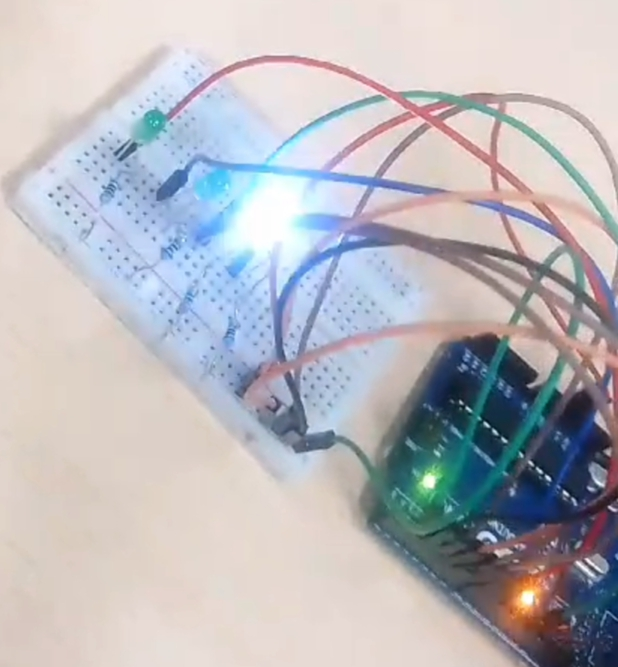
\includegraphics[width=0.4\textwidth]{3.jpg}
 \caption{\label{fig-2:Gates}}               
\end{figure}

\section{CONCLUSION}
 Hence implementation of assembly using LED's is done and verified through truth table.

 \end{document}
